Colocamos la fuente de luz en un extremo del banco y frente a ella la máscara con rendijas, que dejaba pasar siete rayos delgados y paralelos. Sobre la mesa, delante de la máscara, extendimos una hoja blanca para poder ver la trayectoria de los rayos sobre el papel.

Después pusimos la pieza de acrílico.

La acomodamos sobre la hoja, de pie sobre una de sus caras planas, de manera que los siete rayos golpearan su costado curvo y el rayo del centro pasara justo por la mitad del cilindro. Con las luces apagadas, observamos cómo entraban los rayos, cómo salían por el otro lado y en qué zona se cruzaban, y movimos ligeramente la pieza a un lado y a otro para ver si el patrón cambiaba. La figura \ref{fig:frente} muestra el arreglo visto desde la fuente.

\begin{center}
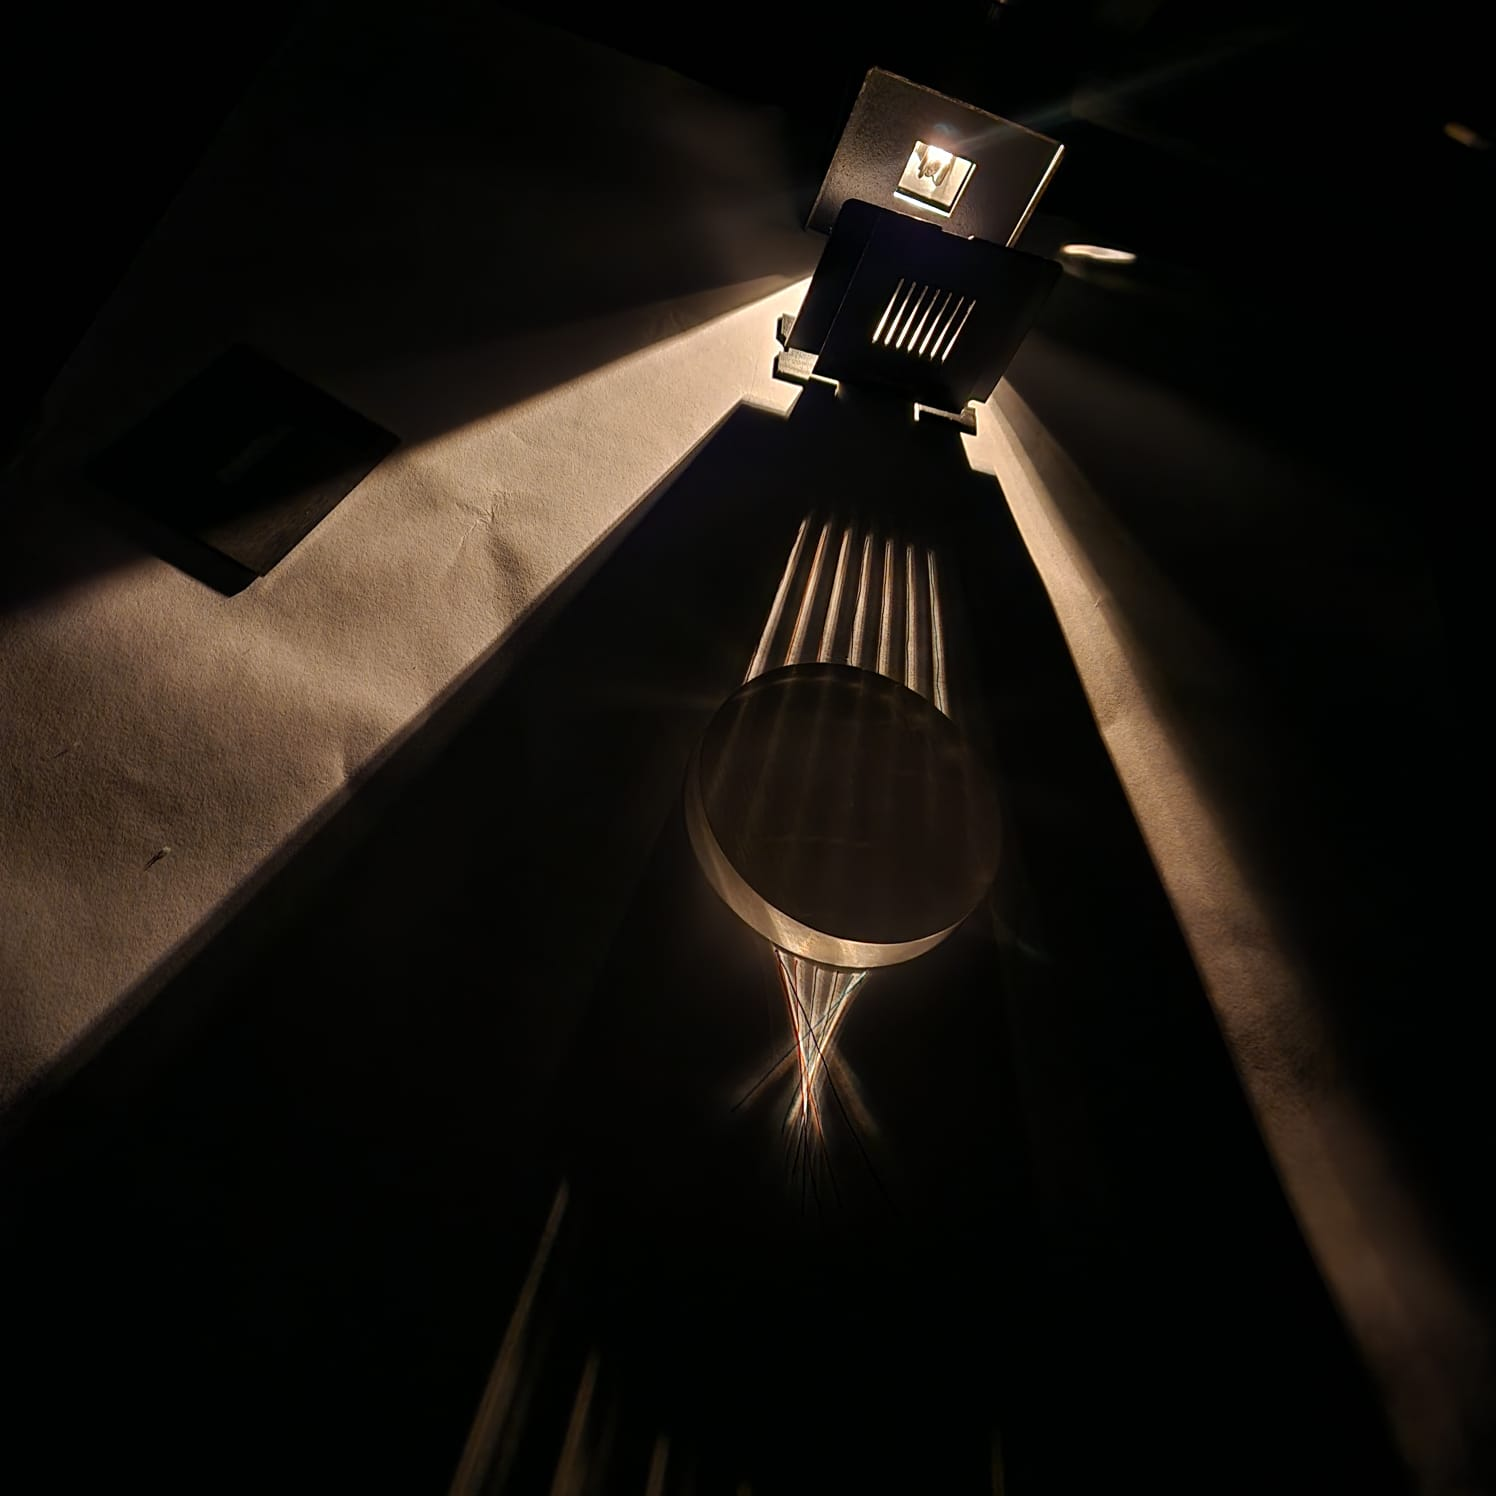
\includegraphics[width=\columnwidth]{rayos_frente.jpg}
\captionof{figure}{Arreglo experimental. Los siete rayos paralelos salen de la máscara, atraviesan el cilindro de acrílico y se cruzan detrás de él.}
\label{fig:frente}
\end{center}

Como no se tomaron medidas, todo lo que sigue se basa en la observación directa y en las fotografías.
